\section{Verification of consistency}

We use NuSMV symbolic model-checker to verify consistency of use-cases with regard to their temporal annotations.
Although NuSMV support BDD-based\footnote{Using binary decision diagrams} and BMC-based\footnote{Bounded model-checking using a SAT solver} model-checking techniques, in our project we use just the BDD-based approach.
NuSMV supports analysis of synchronous and asynchronous systems using Computation Tree Logic (CTL) and Linear Temporal Logic (LTL).
Our framework supports both CTL and LTL, however CTL is preferred because NuSMV would converts LTL formulae into CTL internally.

All use-cases from our UC model have to be converted into NuSMV input language.
We use XText as a tool for handling DSLs (domain specifica languages) which in this case is the NuSMV input language.
NuSMV input language is described using EBNF grammar and XText generates EMF-based model (in-memory representation), language parser and serializer from the grammar.

In order to convert our UC model into NuSMV input language, we use the model-to-model (M2M) approach.
For  transformation between use-case model into generated EMF-model representing the AST of the NuSMV code represented in memory using EMF.

Then the generated serializer produces a valid NuSMV code.

\begin{figure}
  \centering
  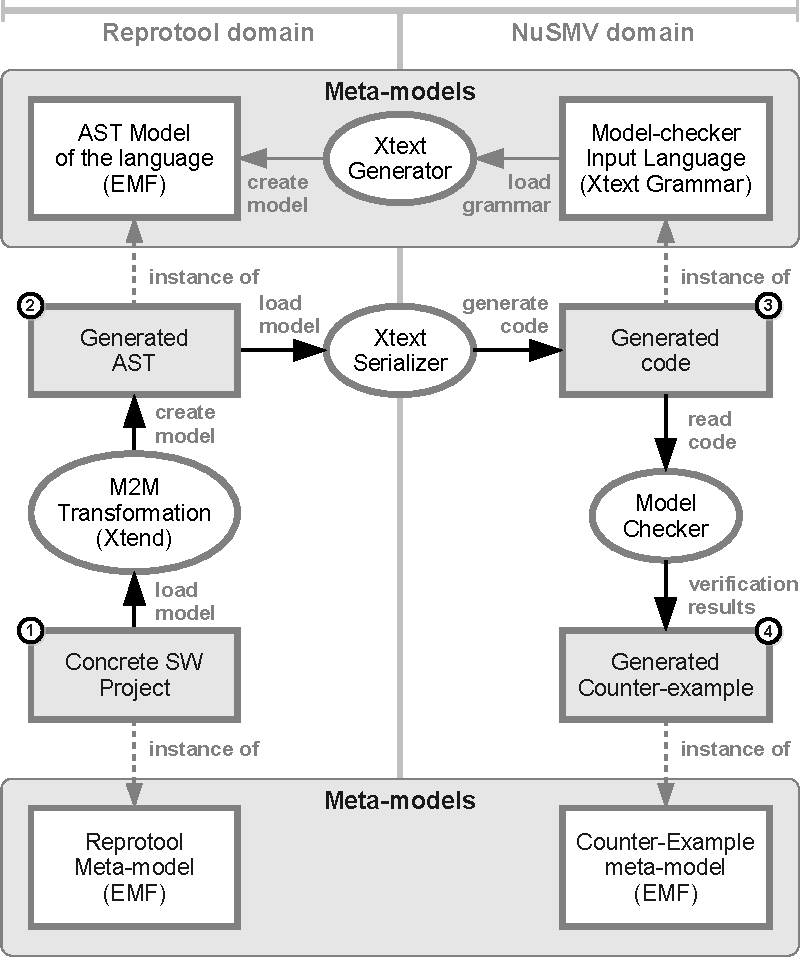
\includegraphics[height=200pt]{images/XtextWorkflow}
  \caption{Transformation of a SW Project into the input language of a model checker}
  \label{fig:XtextWorkflow}
\end{figure}
